% Options for packages loaded elsewhere
\PassOptionsToPackage{unicode}{hyperref}
\PassOptionsToPackage{hyphens}{url}
%
\documentclass[
]{book}
\usepackage{amsmath,amssymb}
\usepackage{lmodern}
\usepackage{iftex}
\ifPDFTeX
  \usepackage[T1]{fontenc}
  \usepackage[utf8]{inputenc}
  \usepackage{textcomp} % provide euro and other symbols
\else % if luatex or xetex
  \usepackage{unicode-math}
  \defaultfontfeatures{Scale=MatchLowercase}
  \defaultfontfeatures[\rmfamily]{Ligatures=TeX,Scale=1}
\fi
% Use upquote if available, for straight quotes in verbatim environments
\IfFileExists{upquote.sty}{\usepackage{upquote}}{}
\IfFileExists{microtype.sty}{% use microtype if available
  \usepackage[]{microtype}
  \UseMicrotypeSet[protrusion]{basicmath} % disable protrusion for tt fonts
}{}
\makeatletter
\@ifundefined{KOMAClassName}{% if non-KOMA class
  \IfFileExists{parskip.sty}{%
    \usepackage{parskip}
  }{% else
    \setlength{\parindent}{0pt}
    \setlength{\parskip}{6pt plus 2pt minus 1pt}}
}{% if KOMA class
  \KOMAoptions{parskip=half}}
\makeatother
\usepackage{xcolor}
\usepackage{longtable,booktabs,array}
\usepackage{calc} % for calculating minipage widths
% Correct order of tables after \paragraph or \subparagraph
\usepackage{etoolbox}
\makeatletter
\patchcmd\longtable{\par}{\if@noskipsec\mbox{}\fi\par}{}{}
\makeatother
% Allow footnotes in longtable head/foot
\IfFileExists{footnotehyper.sty}{\usepackage{footnotehyper}}{\usepackage{footnote}}
\makesavenoteenv{longtable}
\usepackage{graphicx}
\makeatletter
\def\maxwidth{\ifdim\Gin@nat@width>\linewidth\linewidth\else\Gin@nat@width\fi}
\def\maxheight{\ifdim\Gin@nat@height>\textheight\textheight\else\Gin@nat@height\fi}
\makeatother
% Scale images if necessary, so that they will not overflow the page
% margins by default, and it is still possible to overwrite the defaults
% using explicit options in \includegraphics[width, height, ...]{}
\setkeys{Gin}{width=\maxwidth,height=\maxheight,keepaspectratio}
% Set default figure placement to htbp
\makeatletter
\def\fps@figure{htbp}
\makeatother
\setlength{\emergencystretch}{3em} % prevent overfull lines
\providecommand{\tightlist}{%
  \setlength{\itemsep}{0pt}\setlength{\parskip}{0pt}}
\setcounter{secnumdepth}{5}
\usepackage{booktabs}
\usepackage[font=small,labelfont=bf]{caption}
\usepackage{titlesec}
\usepackage{lipsum}

\titleformat{\chapter}[display]
  {\bfseries\Large}
  {\filright\MakeUppercase{\chaptertitlename} \Huge\thechapter}
  {1ex}
  {\titlerule\vspace{1ex}\filleft}
  [\vspace{1ex}\titlerule]
  \pagebreak

\ifLuaTeX
  \usepackage{selnolig}  % disable illegal ligatures
\fi
\usepackage[]{natbib}
\bibliographystyle{apalike}
\IfFileExists{bookmark.sty}{\usepackage{bookmark}}{\usepackage{hyperref}}
\IfFileExists{xurl.sty}{\usepackage{xurl}}{} % add URL line breaks if available
\urlstyle{same} % disable monospaced font for URLs
\hypersetup{
  pdftitle={Baseline risk in medical decision making},
  pdfauthor={Alexandros Rekkas},
  hidelinks,
  pdfcreator={LaTeX via pandoc}}

\title{Baseline risk in medical decision making}
\usepackage{etoolbox}
\makeatletter
\providecommand{\subtitle}[1]{% add subtitle to \maketitle
  \apptocmd{\@title}{\par {\large #1 \par}}{}{}
}
\makeatother
\subtitle{From outcome prediction to the assessment of treatment effect heterogeneity}
\author{Alexandros Rekkas}
\date{}

\begin{document}
\maketitle

{
\setcounter{tocdepth}{0}
\tableofcontents
}
\hypertarget{welcome}{%
\chapter*{Welcome}\label{welcome}}

This is the website for the PhD thesis titled ``\emph{Baseline risk in decision
making: From outcome prediction to the assessment of treatment effect
heterogeneity}''. Visit the \href{https://github.com/rekkasa/thesis}{github
repository} for more information.

\hypertarget{introduction}{%
\chapter{Introduction}\label{introduction}}

\vspace*{\fill}\par
\pagebreak

\hypertarget{personalizing-outcome-risk}{%
\section{Personalizing outcome risk}\label{personalizing-outcome-risk}}

Baseline risk---the probability of a patient experiencing an outcome of interest
without receiving the treatment under study based on a set of predifined
baseline characteristics---is a crucial component of medical decision making.
For example, in the European Society of Cardiology and the European Society of
Hypertension guidelines of 2018 for the management of arterial hypertension,
treatment initiation is based---among other things---on the patient's baseline
10-year cardiovascular risk
{[}\url{https://doi.org/10.1093/eurheartj/ehy339}{]}. Similarly, an algorithm for
management of osteoporosis has been suggested, based on a patient's osteoporotic
fracture risk {[}\url{https://doi.org/10.1007/s00198-019-05176-3}{]}.

Risk prediction models, i.e.~mathematical functions relating the presence of the
outcome of interest to a set of measured predictors (covariates)
{[}\url{https://heart.bmj.com/content/98/9/683}{]}, are important empirical tools for the
assessment of a patient's baseline risk. Adequate evaluation of the prediction
models' performance in new patients is crucial. In most cases, this mainly
focuses on the prediction models' discriminative performance, i.e.~their ability
to separate lower from higher risk patients, and their calibration, i.e.~the
agreement of predicted risk to observed event rates {[}Ewout book; TRIPOD{]}. Though
measures of discrimination and calibration are useful for assessing the
predictive performance of one or multiple prediction models, they do not provide
insight on the added value of using these models for medical decision
making. Baseline risk is only one of the crucial pieces required for predicting
individual responses to treatment. Knowledge of the patients' responsiveness to
treatment, their vulnerability to side-effects and their utilities for other
relevant outcomes is necessary information required for making truly informed
clinical decisions {[}Kravitz, 2004{]}.

\hypertarget{personalizing-treatment-effect}{%
\section{Personalizing treatment effect}\label{personalizing-treatment-effect}}

In order to provide the most optimal medical care, doctors are advised to align
their clinical practice with the results of well-conducted clinical trials, or
the aggregated results from multiple such trials {[}Greenfield 2007{]}. This
approach implicitly assumes that all patients eligible for treatment experience
the same effects (benefits and harms) of treatment as the reference trial
population. However, the estimated treatment effect is often an average of
heterogeneous treatment effects and, as such, may not be applicable to most
patient subgroups, let alone individual patients. If a treatment causes a
serious adverse event, then treating all patients on the basis of an observed
overall positive treatment effect may be harmful for some {[}Rothwell, Lancet
1995; \ldots{]}.

Conceptually, heterogeneity of treatment effect (HTE) is the variation of
treatment effects on the individual level across the population
{[}\url{https://doi.org/10.1111/j.0887-378X.2004.00327.x}{]}. The identification and
quantification of HTE is crucial for guiding medical decision making and lies at the
core of patient-centered outcomes research. Despite HTE being widely
anticipated, however, its evaluation is not straightforward. Individual
treatment effects are---by their nature---unobservable: the moment a patient
receives a specific treatment, their response under the alternatives becomes
unmeasurable (fundamental problem of causal inference; {[}Holland, 1986{]}).

To ``glimpse'' at a specific individual's response under alternative treatments,
researchers usually observe the outcomes of other ``similar'' patients that
actually received one of the other candidate treatments. More individualized
treatment effects are derived from the average effects estimated within a
subgroup of similar patients. However, patient similarity is not straightforward
to assess. Patients differ in a vast number of characterstics which may or may
not be relevant to modifying treatment responses. Identification of such patient
characterstics can be quite complicated. In clinical trials it usually relies on
the detection of statistically significant interactions of treatment with
measured covariates (subgroup analyses).

As clinical trials are usually only adequately powered to detect overall effects
of a certain size, this kind of analyses can be problematic. Existing guidance
on carrying out subgroup analyses attempts to mitigate these issues {[}refs{]}. Lack
of statistical power often results in falsely concluding ``consistency'' of the
treatment effect across several subpopulations of interest or overestimating the
effect size of a treatment-covariate interaction. The former because an existing
interaction effect was smaller than the detectable effect size, the latter
because of false positives introduced from multiple testing. In Figure
\ref{fig:power} the statistical power for detecting an interaction effect of
equal size to the main effect is below 30\%, despite the clinical trial being
powered at 80\% for the detection of the overall effect.

\begin{figure}
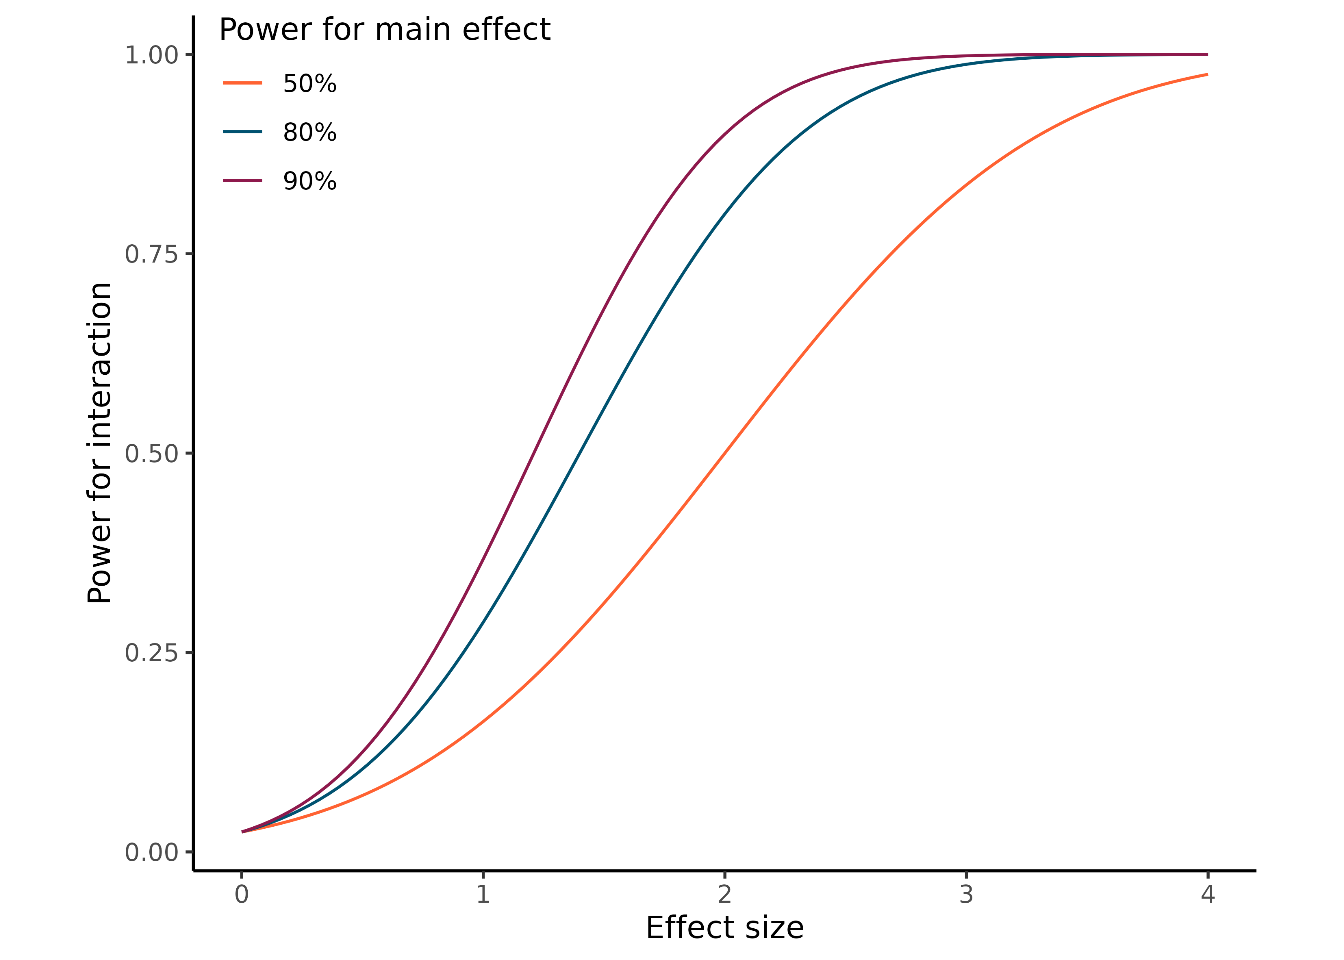
\includegraphics[width=1\linewidth]{Thesis_files/figure-latex/power-1} \caption{Statistical power for the detection of an interaction when the interaction effect size is between 0 and 4 times the main effect size. For simplicity, we assume equal number of treated and untreated patients and that patients are equally separated between the subgroup levels}\label{fig:power}
\end{figure}

Baseline risk is an important determinant of treatment effect {[}refs{]}. It sets an
upper bound on the treatment effect size. Low risk patients can only experience
minimal treatment benefit before their risk is reduced to zero, while high risk
patients can benefit much more. This means that baseline risk can be used as a
subgrouping variable for assessing HTE. For many common settings prediction
models of high quality for estimating baseline risk already exist and can be
directly applied to the data at hand {[}refs{]}. If no such models exist, the
researcher can develop one from the available dataset {[}refs{]}.

Baseline risk can also be used for directly predicting individual treatment
benefit {[}Califf; Dahabreh, IJE 2016{]}. For example Califf et al {[}ref{]} predicted
individual benefits regarding mortality with tissue plasminogen activator (tPA)
compared to streptokinase treatment in patients with acute myocardial infarction
using baseline mortality risk and assuming a constant relative tPA treatment
effect. However, relative treatment effect does not need to be assumed
constant. Modeling more flexible interactions of treatment with baseline outcome
risk may provide more informative absolute benefit predictions for individual
patients.

Depending on the scale treatment effect is measured, HTE may or may not be
identified (Figure \ref{fig:scale}). For example, despite finding statistically
significant subgroup effect evaluated on the relative scale, the absolute risk
difference between the two groups may be so small that has no clinical relevance
{[}\url{http://dx.doi.org/10.1016/j.jclinepi.2013.11.003}{]}. Therefore, in the presence
of a truly effective treatment, effect heterogeneity should always be
anticipated on some scale {[}Dahabreh, IJE 2016{]}, as baseline risk is bound to
vary across trial patients. If effect modifiers are known and the available
sample size provides adequate statistical power for evaluating
treatment-covariate interactions, modeling these interactions would be the
optimal approach for assessing HTE. However, this approach may lead to
overfitting and unstable estimates for the interaction effects {[}Balan, JCE{]}.

\begin{figure}
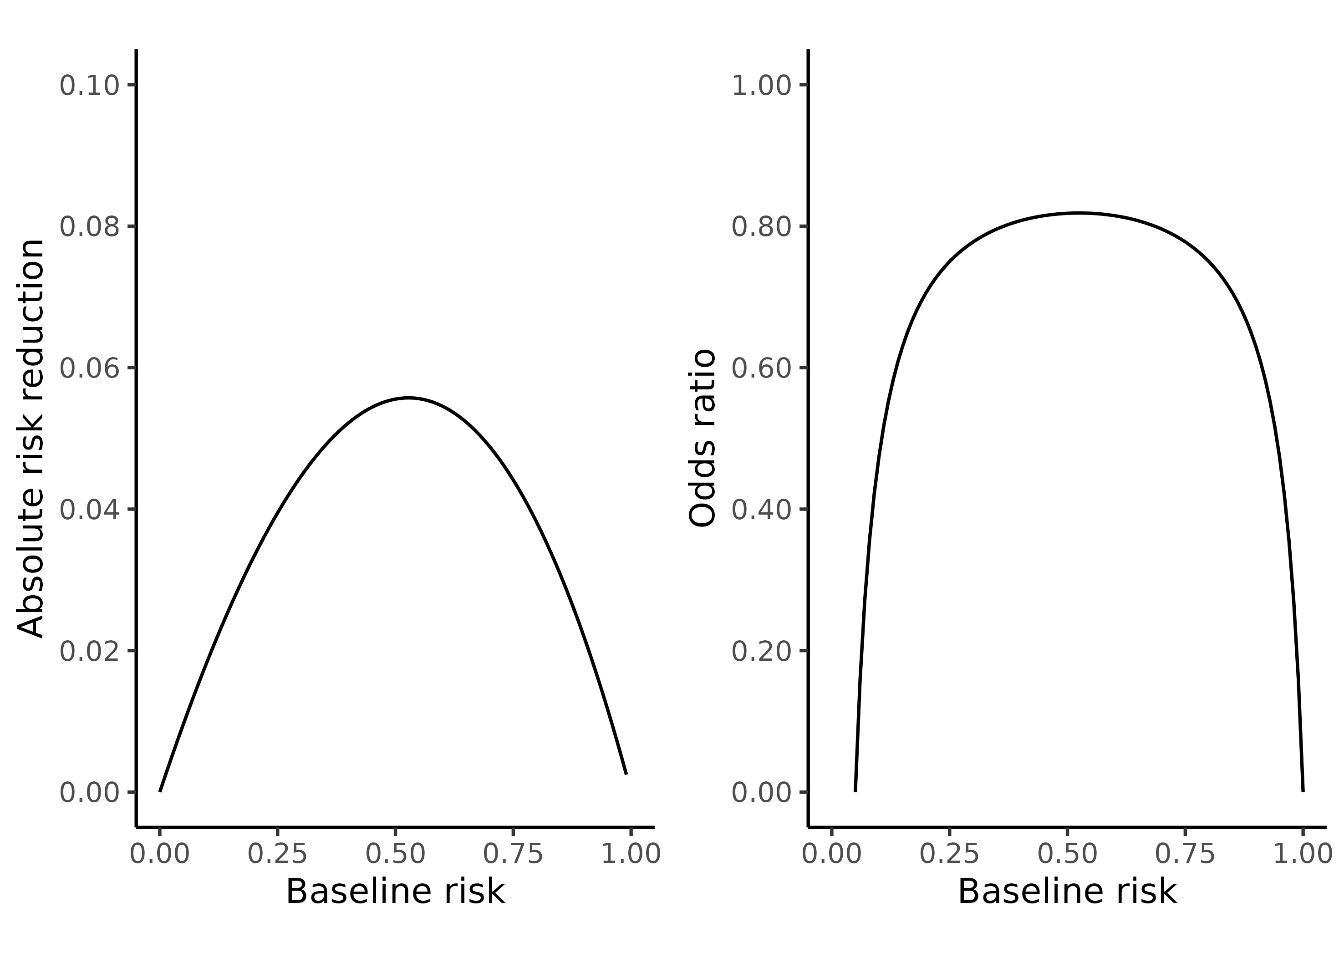
\includegraphics[width=1\linewidth]{Thesis_files/figure-latex/scale-1} \caption{Scale dependency of treatment effect heterogeneity. In the left panel a constant odds ratio of 0.8 is assumed. In the right panel a constant absolute risk reduction of 0.1 is assumed.}\label{fig:scale}
\end{figure}

\hypertarget{observational-data}{%
\section{Observational data}\label{observational-data}}

Healthcare data is routinely collected by general practitioners, hospitals,
insurance companies, and many other private or public bodies and is becoming
increasingly available giving researchers access to massive amounts of patient
data. Theoretically, the aforementioned statistical power challenges for the
evaluation of HTE would be largely mitigated if the analyses were performed on
even a single such database. However, as this data is not being accumulated for
research purposes, it suffers from many biases causing many commonly used
methods to fail. Doctors prescribing a specific treatment expect---usually based
on results from clinical trials---that it will be beneficial for the patient
they are treating. This causes systematic differences in important
characteristics among patients receiving different treatments and renders their
comparison very challenging.

If all relevant patient characteristics on which the treating physician based
their decision have been captured in the observational dataset, methods are
available that can be used to account for these systematic differences
{[}refs{]}. Among the more popular ones is limiting the analyses to the propensity
score matched subpopulation. Propensity scores are the patient-specific
probabilities of receiving the treatment under study and have been shown to have
the balancing property, i.e.~conditional on the propensity score treatment
assignment is independent of the potential outcomes {[}refs{]}. This means that in a
subset of patients with equal propensity scores there are no differences in
covariate distributions between patients receiving the treatment under study and
those who are not. Consequently, patients within this subset can be assumed to
be randomized.

Unfortunately, not all the information that was used to decide on treatment is
captured. As a consequence, propensity score adjustment will not suffice to
evaluate treatment effects using the observational data, be it overall or
subgroup effects. Sensitivity analyses searching for evidence of this systematic
unmeasured imbalances have been proposed and can be of assistance in many
situations {[}refs{]}.

Another important problem with observational databases is that they use
different architectures. As anyone gathering routinely observed healthcare data
did so in a way that was more convenient to them, a plethora of structures for
the resulting databases arose. Diseases, treatments, medical exams and many more
aspects of healthcare are often coded differently in different observational
databases. In addition, more fundamental disparities between databases also
factor in database incopatibility: different types of information are recorded
in different databases. Different patient characteristics are captured---at
different levels of detail---in a general practitioner database, in a hospital
medical record or in an administrative claims database. This means that
combining results from multiple databases is not a simple task.

One of the solutions put forward for handling database incompatibility was the
creation of the Observational Medical Outcomes Partnership Common Data Model
(OMOP-CDM) {[}refs{]}. This provided a standard for structuring an observational
database while large effort was put into developing processes for mapping
existing databases from their own specific structure to OMOP-CDM. A high level of
standardization and scalability for observational studies was achieved. Common
definitions of diseases, treatments, and outcomes can now be applied uniformly
across a network of many databases containing information on hundreds of
millions of patients. An analysis plan can be executed following the exact same
steps across the network providing effect estimates derived in different
populations. The fragmented information scattered across multiple databases can
now be summarized in a consistent way to give a fuller picture.

The power of the common database structure was demonstrated in a large-scale
comparative effectiveness study of first-line treatment for hypertension
{[}Suchard, Lancet 2019{]}. This study compared five different first-line drug
classes prescribed for hypertension regarding three primary effectiveness, six
secondary effectiveness, and 46 safety outcomes across a global network of 9
observational databases, all mapped to OMOP-CDM. A framework following best
practices for carrying out such analyses was proposed and implemented on a large
scale. The results complemented the already available evidence generated in
clinical trials, confirming earlier findings and providing effect estimates on
previously unexplored comparisons.

Observational databases provide access to massive numbers of ``real-life''
patients. This motivates the exploration of methods for the assessment of
treatment effect heterogeneity in the observational setting despite the
challenges inherent to this type of data. The statistical power problem related
to multiple subgroup analyses can still be present, as observational data is
high-dimensional, i.e.~the number of measured patient characteristics increases
with the number of patients. Attempting a treatment effect modeling approach,
where treatment-covariate interactions are modeled for the prediction of
individualized treatment benefits, suffers from the same statistical power
issues and often results to highly variable estimates. Therefore, using baseline
outcome risk as the subgrouping variable, can provide good insight of treatment
effect heterogeneity in the observational setting. Modern libraries for
developing risk prediction models and for correcting for confounding are
available and---capitalizing on OMOP-CDM---can be easily applied across
databases with millions of patients.

\hypertarget{aims}{%
\section{Aims}\label{aims}}

The overall aim of this thesis is to explore the use of baseline risk prediction
models as the basis for medical decision making. We will study and apply methods
for the evaluation of treatment effect heterogeneity in both clinical trial data
and observational data. The specific research aims are:

\begin{enumerate}
\def\labelenumi{\arabic{enumi}.}
\tightlist
\item
  \emph{Systematically organize the current literature on predictive approaches to
  treatment effect heterogeneity}. We are going to focus on regression modeling
  approaches applied in clinical trial data. Methods will be categorized based
  on their definition of patient similarity.
\item
  \emph{Develop risk-based predictive approaches to the assessment of treatment
  effect heterogeneity}. We are going to explore new subgrouping methods based
  on risk stratification along with more personalized approaches, focusing on
  both the observational and clinical trial setting. Scalability and
  reproducibility of the considered methods are crucial.
\item
  \emph{Apply risk-based methods to better guide medical decisions}. We are going to
  develop baseline risk prediction models in several case studies easily
  applicable in clinical practice.
\end{enumerate}

In \textbf{Chapter 2} we present the results of a scoping literature review of
regression modeling approaches for the assessment of treatment effect
heterogeneity in the clinical trial setting. The identified methods are divided
into broader categories based on how they incorporate prognostic factors and
treatment effect modifiers.

In \textbf{Chapter 3} we develop a standardized scalable framework for the assessment
of treatment effect heterogeneity using a risk-stratified approach in the
observational setting. We, also, develop the software for the execution of the
framework in observational databases mapped to OMOP-CDM. We, finally,
demonstrate the application of the framework, assessing treatment effect
heterogeneity in first-line treatment for hypertension across three US claims
databases.

In \textbf{Chapter 4} we compare different risk-based methods for predicting
individualized treatment effects using an extensive simulation study. We only
consider the clinical trial setting were treatment is admistered at random.

In \textbf{Chapter 5} we develop a model for the prediction of 5-year recurrence risk
in sentinel node positive melanoma patients, using data from nine European
Organization for Research and Treatment of Cancer centers. We calibrate the
recurrence model to predict 5-year risk of distant metastasis and overall
mortality and develop a nomogram for graphical representation. The models are,
then, extenrally validated.

In \textbf{Chapter 6} we develop a model for the prediction of 28-day mortality for
patients presenting at the emergency department with suspected COVID-19
infection at four large Dutch hospitals between March and August, 2020. We
predict 28-day admission to the intensive care unit by calibrating the mortality
model. An easy to use web application is also supplied. We perform temporal
validation to assess model performance using data between September and
December, 2020.

In \textbf{Chapter 7} we apply the standardized framework to evaluate effect
heterogeneity of teripatide treatment compared to oral bisphosphonates in female
patients above the age of 50 with established osteoporosis. We use different
risk stratification approaches based on quantiles of predicted risk and
externally derived risk thresholds for treatment. We evaluate the presence of
residual confounding using sensitivity analyses.

Finally, in \textbf{Chapter 8} we present a general discussion along with
perspectives on future work.

\hypertarget{predictive-approaches-to-heterogeneous-treatment-effects-a-scoping-review}{%
\chapter{Predictive approaches to heterogeneous treatment effects: a scoping review}\label{predictive-approaches-to-heterogeneous-treatment-effects-a-scoping-review}}

\vspace*{\fill}\par
\pagebreak

\hypertarget{a-standardized-framework-for-risk-based-assessment-of-treatment-effect-heterogeneity-in-observational-healthcare-databases}{%
\chapter{A standardized framework for risk-based assessment of treatment effect heterogeneity in observational healthcare databases}\label{a-standardized-framework-for-risk-based-assessment-of-treatment-effect-heterogeneity-in-observational-healthcare-databases}}

\vspace*{\fill}\par
\pagebreak

\hypertarget{sim}{%
\chapter{Individualized treatment effect was predicted best by modeling baseline risk in interaction with treatment assignment}\label{sim}}

\vspace*{\fill}\par
\pagebreak

\hypertarget{the-eortc-decog-nomogram}{%
\chapter{The EORTC-DeCOG nomogram}\label{the-eortc-decog-nomogram}}

\vspace*{\fill}\par
\pagebreak

\lipsum[1-4]

\hypertarget{covid-outcome-prediction-in-the-emergency-department}{%
\chapter{COVID Outcome Prediction in the Emergency Department}\label{covid-outcome-prediction-in-the-emergency-department}}

\vspace*{\fill}\par
\pagebreak

\lipsum[1-4]

\hypertarget{osteoporosis-project}{%
\chapter{Osteoporosis project}\label{osteoporosis-project}}

\hypertarget{discussion}{%
\chapter{General discussion}\label{discussion}}

\vspace*{\fill}\par 
\pagebreak

\hypertarget{organization-of-predictive-treatment-effect-heterogeneity-literature}{%
\section{Organization of predictive treatment effect heterogeneity literature}\label{organization-of-predictive-treatment-effect-heterogeneity-literature}}

\hypertarget{main-findings}{%
\subsection{Main findings}\label{main-findings}}

We systematically organized the available methodological literature on the
evaluation of treatment effect heterogeneity using the reference class each
method used to define patient similarity. This resulted in the identification of
three separate categories of methods.

Risk-based approaches define patient similarity based solely on risk
factors. These methods can be further divided into risk stratification
approaches that rely on the definition of risk-based subgroups of patients and
risk magnification approaches that assume a constant relative treatment
effect. The latter can be used to make personalized benefit predictions. In
chapter \ref{sim} the strong assumtion of constant relative treatment effects
was relaxed, allowing for increasingly flexible (\textbf{??}) interactions of
baseline risk with treatment. Of course, the assumption that treatment effect is
a function of basline risk remained intact.

Treatment effect modeling methods focus both on risk factors and treatment
effect modifiers to make personalized absolute benefit predictions. These
methods are more intuitive, in the sense that they attempt to account for all
dimensions of treatment effect heterogeneity (\textbf{elaborate!!}). However,
statistical power is an important constraint, as multiple treatment-covariate
interaction effects need to be estimated. In the presence of well-documented and
clinically supported effect modifiers statistical power may suffice as only a
small pre-defined set of interaction effects will be evaluated. In more
automated settings, staging or penalization approaches can be considered. The
former rely on the ``calibration'' of first-stage ``working'' models including many
treatment-covariate interactions. The latter rely on automated processes that
shrink the estimated interaction effects towards 0.

Finally, optimal treatment rule methods focus on modeling treatment effect
modifiers for the evaluation of treatment effect heterogeneity. Their aim is not
to provide personalized treatment effect estimates or to separate patients into
subgroups of similar expected treatment effect, but rather to separate them into
two categories. Patients who benefit from treatment and patients who do not. If
there are no major treatment-related harms, they can be used out of the box to
guide medical decisions. However, in the presence of serious treatment adverse
events, these methods may be more challenging to implement. That is because the
effect of baseline risk factors is not taken into account. This means that the
baseline risk of the main outcome of interest is not evaluated and, therefore,
the absolute risk reduction achieved with treatment cannot be compared to the
risk increase for the adverse event in question. Also, the clinical relevance of
following the treatment assignment rule cannot be easily evaluated
(\textbf{elaborate!!}).

\hypertarget{limitations}{%
\subsection{Limitations}\label{limitations}}

A large number of methods have been suggested in medical research for the
evaluation of treatment effect heterogeneity. However, treatment effect
heterogeneity is not a problem specific to healthcare research with important
advances being made in economics, social sciences, and other fields, as well. In
addition, the increasing availability of observational data from massive
databases capturing a large proportion of patients' interaction with the
healthcare system has provided additional challenges, with confounding,
suboptimal data capture, local or temporal inconsistencies only being a few of
them. All these have resulted on the suggestion of many different methods for
the evaluation of treatment effect heterogeneity, many of which may have not
been captured in our literature review. Our focus was on the clinical trial
setting and mainly regression-based methods were considered.

The above categorization of methods for the assessment of treatment effect
heterogeneity is not the only possible. When focusing on subgroup analyses
\href{https://onlinelibrary.wiley.com/doi/full/10.1002/sim.7064}{Lipkovich et al}
identified two frameworks for personalized medicine: 1) methods that identify
the right patient for a specific treatment and 2) methods that identify the
right treatment for a specific patient. In the first case, a set of treatment
effect modifiers is sought that quantitavely interact with treatment in an
attempt to achieve the highest overall benefit across the entire population. In
the second case, the objective is the idertification of a set of effect
modifiers that qualitatively interact with treatment.

In a more technical approach focusing mainly on tree-based methods,
\href{https://doi.org/10.1073/pnas.1804597116}{Kunzel} separated existing staging
methods into A and S-learners while also suggesting a new approach, the
X-learners. The suggested methods differred in the way they used to recalibrate
the initially derived estimates to estimate conditional average treatment
effects. Assuming binary treatment assignment, A-learners fit treatment-arm
specific models before estimating individualized treatment effects as their
difference. S-learners include treatment assignment in the development of the
tree-based model. They estimate conditional average treatment effect as the
differnce of between setting the treatment indicator to control and active
treatment. Finally, their proposed X-learners, use first-stage outcome models
separately fitted in each treatment arm to impute coutnerfactual outcomes, thus
generating an ``observed'' treatment effect. Any regular modeling approach can
then be used to estimate treatment effects.

\hypertarget{future-research}{%
\subsection{Future research}\label{future-research}}

Future research should attempt to better capture the expanding literature, and
adequately summarize it to identify gaps and also cross-pollinate
(\textbf{rephrase!!}) among the different fields working on what essentially can be
seen as the same problem (\textbf{rephrase!!}). The categorization methods provided
here could help (\textbf{continue!!})\ldots{}

\end{document}
